\thispagestyle{plain}
\chapter{Kosmische Strahlung}
In diesem Kapitel wird die kosmische Strahlung beschrieben, welche die Erdatmosphäre erreicht. Die kosmische Strahlung kann in eine primäre und eine sekundäre Komponente zerlegt werden. Die primäre Komponente beschreibt alle Teilchen, welche die Erdatmosphäre erreichen, wohingegen die sekundäre Komponente alle Teilche sind, welche von dem Primärteilchen während der Propagation zur Erdoberfläche produziert werden und auf der Erde detektiert werden können.
 
\section{Primäre kosmische Strahlung S.5}
\begin{figure}[!h]
    \centering
    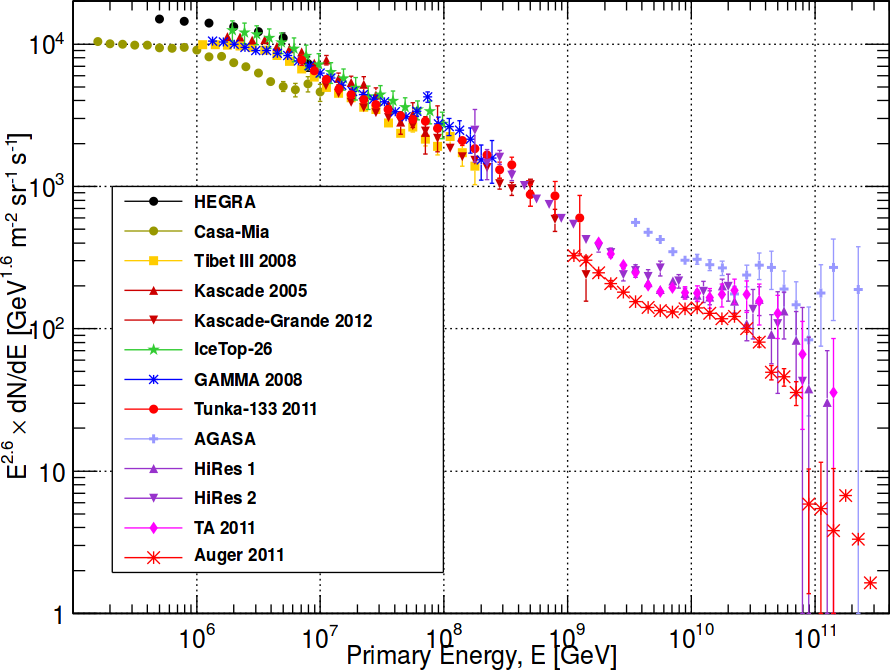
\includegraphics[width=0.7\textwidth]{./Plots/CR_Spectrum.png}
    \caption{Differentielles Spektrum der kosmischen Strahlung gemessen durch verschiedenen Exterimente.\ref{Paper} Dieses Spektrum ist mit der Energie, um einen Faktor von $E^{2.6}$ gewichtet. Dadurch sind das Knie ($\approx$\SI{3}{PeV}), das zweite Knie ($\approx$\SI{80}{PeV}) und die Ferse ($\approx$\SI{50}{EeV}) des Spektrums der Kosmischen Strahlung deutlich erkennbar.}
    \label{fig:SpecStrahl}
\end{figure}
\section{Sekundäre kosmische Strahlung S.2}
\section{Prompte Leptonen S.3-4}